% !TEX root = ../main_lecture_notes.tex
\chapter{Introduction}\label{sec:introduction}

A blockchain is a distributed ledger made of a sequence of blocks maintained by achieving consensus among a number of nodes in a Peer-to-Peer network. The blockchain technology has attracted a lot of interest after the advent of the bitcoin cryptocurrency in 2008, see \citet{Na08}. Since then, the blockchain concept has been used to develop decentralized systems to store and maintain the integrity of time-stamped transaction data across peer-to-peer networks. Besides the creation of a digital currency, blockchain applications include the sharing of IT resources, the registration of authentication certificate or the implementation of smart contracts. \\

\noindent A blockchain is 
\begin{itemize}
	\item Decentralized as it is maintained by a network. Nodes can be light or full nodes. Light nodes are blockchain users that broadcast transactions, full nodes are in charge of verifying and recording the transactions, see \cref{fig:blockchain_network}.
	\begin{figure}[ht!]
\begin{center}
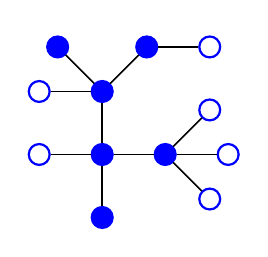
\begin{tikzpicture}[-, >=, auto, semithick, node distance=01cm]
\tikzstyle{every edge}=[segment length=1mm,segment angle=10, draw]

\tikzstyle{full node}=[circle, fill=blue,draw=blue,thick,text=black,scale=0.8]
\tikzstyle{light node}=[circle, fill=white,draw=blue,thick,text=black,scale=0.8]
\node[full node]    (1)                     {};
\node[full node]    (2)[above right of=1]         {};
\node[full node]    (3)[above left of=1]         {};
\node[full node]    (4)[below of=1]         {};
\node[full node]    (5)[right of=4]         {};
\node[full node]    (6)[below of=4]         {};
\node[light node]    (7)[left of=1]         {};
\node[light node]    (8)[right of=2]         {};
\node[light node]    (9)[left of=4]         {};
\node[light node]    (10)[above right of=5]         {};
\node[light node]    (11)[ right of=5]         {};
\node[light node]    (12)[ below right of=5]         {};
% \node[light node]    (4)[above of=2]         {};
\path

(1) edge node{} (2)
    edge node{} (3)
    edge node{} (7)
    ;
\path
(5) edge node{} (10)
    edge node{} (11)
    edge node{} (12)
    ;
    \path
(4) edge node{} (5)
    edge node{} (1)
    edge node{} (9)
    edge node{} (6)
    ;
    \path
(2) edge node{} (8)   
    ;
\end{tikzpicture}
\end{center}
\caption{A network made of full nodes (blue) and light nodes (white)}
\label{fig:blockchain_network}
\end{figure}

	\begin{itemize}
		\item A local copy is stored by each full node which grants security
		\item The governance is not handled by a central authority
	\end{itemize}
	\item Public or private. In public blockchain anyone can access the data, in private blockchain reading access is restricted.
	\item permissionned or permissionless. In permissionless blockchain, anyone can join the network as a full node.
	\item Immutable. Altering the information written in the blockchain is made difficult if not impossible.
	\item Incentive compatible. The process of reaching consensus is costly to the full nodes who must be compensated for their hard work.
\end{itemize}
The consensus protocols, at the core of the blockchain technologies, are the focus of these lecture notes. The goal is to evaluate consensus protocol according to three dimensions 
\begin{enumerate}
	\item Efficiency: The amount of data being processed per time unit
	\item Decentralization: The fairness of the distribution of the decision power among the nodes
	\item Security: The likelihood of a successful attack on the blockchain
\end{enumerate}
Because consensus protocols involve random components, stochastic modelling is required to assess a blockchain system within the Efficiency/Decentralization/Security trilemma in \cref{fig:blockchain_trilemma}. 
\begin{figure}[ht!]
\begin{center}
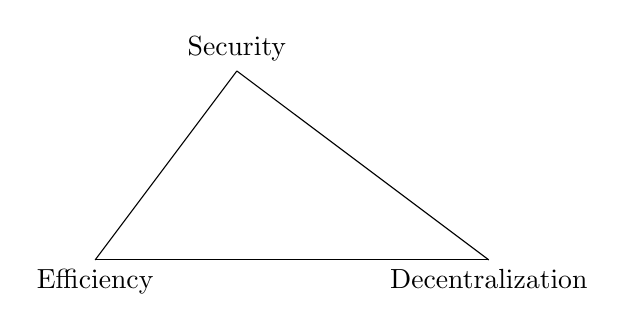
\begin{tikzpicture}
\draw (0,0) -- (5,0); % AB = 5
\draw (0,0) node [below] {Efficiency};
\draw (0,0) -- (1.8,2.4); % AC = 3
\draw (5,0) node [below] {Decentralization};
\draw (5,0) -- (1.8,2.4); % BC = 4
\draw (1.8,2.4) node [above] {Security};
\end{tikzpicture}
\end{center}
\caption{The blockchain trilemma}
\label{fig:blockchain_trilemma}
\end{figure}
As it is hard to improve one dimension without negatively impacting the other two, trade-offs must be made. We will see how to use classical models of applied probability, including urn, epidemic, graph, queue and risk models, to provide numerically tractable indicators to quantify the efficiency, decentralization and security of blockchain systems. These indicators will then allow us to carry out sensitivity analysis with respect to the model parameters to optimize and improve blockchain implementations.\\

\noindent The main application of blockchain systems today is undoubtedly cryptocurrencies, the most well known of which being the bitcoin introduced by \citet{Na08}. Public and permissionless blockchain, like the bitcoin one, must be associated to a cryptocurrency. Indeed, to add a block to the bitcoin blockchains the full nodes compete to solve a cryptrographic puzzle using brute force search algorithm. The first node (referred to as a miner) who finds a solution, appends the next block and collects a reward expressed in cryptocurrency. Assuming this reward is worth something, it offsets the operational cost which is essentially the electricity consumed to run the computers 24/7. A cryptocurrency must be equipped with following features
\begin{enumerate}
  \item No central authority (Decentralized network)
  \item Ledger to record all the transactions and coin ownership (the blockchain)
  \item A coin generation process (block finding reward)
    \begin{itemize}
    \item[$\hookrightarrow$] It creates an incentive compatible system to the full nodes 
  \end{itemize}
  \item Ownership can be proved cryptographically, a wallet is secured with a public/private key system 
  \item Transactions can be issued by an entity proving ownership of the cryptographic unit through the private key
  \item The system cannot process more than one transaction associated to the same cryptographic unit. It must be robust to double spending attack in which a fraudster is issuing two conflicting transactions to recover the funds she already spent
\end{enumerate}
This charcaterization is given by \citet{Lansky2018}.
Cryptocurrencies draw their fundamental value from the fact that they 
\begin{itemize}
  \item provide transaction anonymity
  \item provide a reliable currency in certain regions of the world
  \item permit money transfer worldwide at low fare
  \item do not require a thrusted third party
\end{itemize} 
An important implication of this architecture is disintermediation, it creates an environment where
multiple parties can interact directly and transparently. Blockchain is therefore immediately relevant
to banks and financial institutions which incur huge middlemen costs in settlements and other back office operations. Decentralized finance (DeFi) offers a new financial architecture that is non-custodial, permissionless, openly auditable, pseudo-anonymous and with potential new capital efficiencies. It extends the promise of the original bitcoin whitepaper \citet{Na08} of non-custodial transaction
to more complex financial operations, see the SoK of \citet{werner2021sok}.\\

\noindent Blockchain is a research topic of interest to many communities. Computing science distributed ledger technologies (synonymous with blockchains) rely on distributed algorithms and enable cooperation within a peer-to-peer network. Linking blocks and checking the authenticity of data uses cryptographic functions which is another field of computer science. The establishment of an incentive system within a network of individuals adopting a strategic behavior naturally leads to problems of game theory similar to those solved by economists. The discussion on the nature of new financial assets such as crypto-currencies, utility tokens and non-fungible tokens, is also at the center of the concerns of researchers in finance and monetary economics. \\

\noindent We focus here on the use of mathematics to optimize blockchain systems which makes our problems very close to those encountered in operations research. These notes are organized as follows. \cref{chap:consensus} presents the various consensus algorithms. \cref{chap:security} focuses on the security aspects. In \cref{chap:security}, we take a look at decentralization in \cref{chap:decentralization}. We close on efficiency with \cref{chap:efficiency}.



The topic of blockchain is of primary interest to computer scientists working on peer-to-peer networks and distributed algorithm. The problem of reaching consensus inside peer-to-peer networks is a classical problem in computer science. A consensus protocol just take advantage of the limited resources of the network which includes
\begin{itemize} 
	\item bandwidth
	\item computational power
	\item storage
\end{itemize}
The most natural solution is to proceed to a majority vote via a system of message exchange. It was proposed a long time ago to solve "The Byzantine general problem" as framed by \citet{lamport1982the} in an abstract way. The issue is that exchanging messages inside a peer-to-peer network that can grow very large is not a practical solution. The colossal number of messages is prohibitive, it leads to communication overhead and the failure of some nodes by denial of service.   

The goal is to find an algorithm which allows the node of the networks to agree despite the presence of crashing nodes and faulty nodes (also referred to as Byzantine node)

A group of generals from the Byzantine army is surrounding an enemy city. Communicating only by messenger, they must agree on a common battle plan. There may be traitors who will attack instead of retreat or non responding generals who will do nothing. For the project to be successful a majority of the general must either retreat or attack. The problem then reduces to finding an algorithm to ensure that the loyal generals reach an agreement. The problem is illustrated on \cref{fig:byzantine_general}.
\begin{figure}[!ht]
  \begin{center}
    \subfloat[Coordinated attack]{
      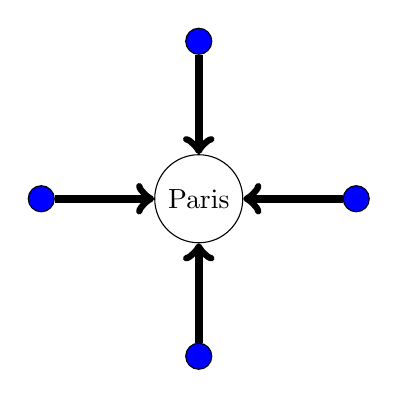
\begin{tikzpicture}[baseline]
\node[draw, circle] (P) at (0,0) {Paris};
\foreach \i in {(0,2), (0,-2), (2,0), (-2, 0)}{
		\node[draw, circle, fill = blue] (G) at \i {};
		\draw[->, line width=1mm,black] (G) -- (P);
	}
\end{tikzpicture}}
                         \hskip2em
    \subfloat[Failed attack due to one traitor and one non-responding general]{
      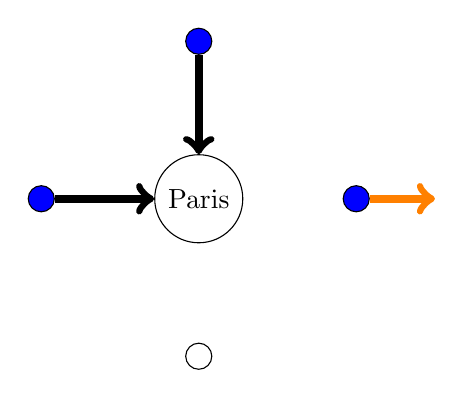
\begin{tikzpicture}[baseline]
\node[draw, circle] (P) at (0,0) {Paris};
\foreach \i in {(0,2),  (-2, 0)}{
		\node[draw, circle, fill = blue] (G) at \i {};
		\draw[->, line width=1mm,black] (G) -- (P);
	}

	\node[draw, circle, fill = blue] (G) at (2,0) {};
	\draw[->, line width=1mm,orange] (G) -- (3,0);
	\node[draw, circle] (G) at (0,-2) {};
\end{tikzpicture}}
    
    \caption{Illustration of the BYzantine general problem}
    \label{fig:byzantine_general}
  \end{center}
  \end{figure}

In a blockchain system, we have a large network of nodes that broadcast transactions which corresponds to pieces of information that will be written in the blockchain. light nodes, full nodes consensus and write information. 


\begin{itemize}
	\item Computer science
	\item Economics
	\item Applied math and operations research
\end{itemize}
\newpage